% Copyright (c) 2022 by Lars Spreng
% This work is licensed under the Creative Commons Attribution 4.0 International License.

\documentclass[
11pt,notheorems,hyperref={pdfauthor=whatever}
]{beamer}

\usepackage{kotex}
\input{loadslides.tex}

\usepackage{fontspec}
\IfFontExistsTF{Pretendard}{%
  \setmainfont[
    UprightFont={Pretendard Medium},
    BoldFont={Pretendard Bold},
    ItalicFont={Pretendard Medium},
    BoldItalicFont={Pretendard Bold}
  ]{Pretendard}
  \setsansfont[
    UprightFont={Pretendard Medium},
    BoldFont={Pretendard Bold},
    ItalicFont={Pretendard Medium},
    BoldItalicFont={Pretendard Bold}
  ]{Pretendard}
  \setmonofont[
    UprightFont={Pretendard Medium},
    BoldFont={Pretendard Bold},
    ItalicFont={Pretendard Medium},
    BoldItalicFont={Pretendard Bold}
  ]{Pretendard}
  \setmainhangulfont[
    UprightFont={Pretendard Medium},
    BoldFont={Pretendard Bold},
    ItalicFont={Pretendard Medium},
    BoldItalicFont={Pretendard Bold}
  ]{Pretendard}
  \setsanshangulfont[
    UprightFont={Pretendard Medium},
    BoldFont={Pretendard Bold},
    ItalicFont={Pretendard Medium},
    BoldItalicFont={Pretendard Bold}
  ]{Pretendard}
  \setmonohangulfont[
    UprightFont={Pretendard Medium},
    BoldFont={Pretendard Bold},
    ItalicFont={Pretendard Medium},
    BoldItalicFont={Pretendard Bold}
  ]{Pretendard}
}{%
\IfFontExistsTF{NanumGothic}{%
  \setmainfont[
    UprightFont=NanumGothicBold,
    BoldFont=NanumGothicBold
  ]{NanumGothic}
  \setsansfont[
    UprightFont=NanumGothicBold,
    BoldFont=NanumGothicBold
  ]{NanumGothic}
  \setmonofont[
    UprightFont=NanumGothicBold,
    BoldFont=NanumGothicBold
  ]{NanumGothic}
  \setmainhangulfont[
    UprightFont=NanumGothicBold,
    BoldFont=NanumGothicBold
  ]{NanumGothic}
  \setsanshangulfont[
    UprightFont=NanumGothicBold,
    BoldFont=NanumGothicBold
  ]{NanumGothic}
  \setmonohangulfont[
    UprightFont=NanumGothicBold,
    BoldFont=NanumGothicBold
  ]{NanumGothic}
}{%
  \IfFontExistsTF{Nanum Gothic}{%
    \setmainfont[
      UprightFont=Nanum Gothic Bold,
      BoldFont=Nanum Gothic Bold
    ]{Nanum Gothic}
    \setsansfont[
      UprightFont=Nanum Gothic Bold,
      BoldFont=Nanum Gothic Bold
    ]{Nanum Gothic}
    \setmonofont[
      UprightFont=Nanum Gothic Bold,
      BoldFont=Nanum Gothic Bold
    ]{Nanum Gothic}
    \setmainhangulfont[
      UprightFont=Nanum Gothic Bold,
      BoldFont=Nanum Gothic Bold
    ]{Nanum Gothic}
    \setsanshangulfont[
      UprightFont=Nanum Gothic Bold,
      BoldFont=Nanum Gothic Bold
    ]{Nanum Gothic}
    \setmonohangulfont[
      UprightFont=Nanum Gothic Bold,
      BoldFont=Nanum Gothic Bold
  ]{Nanum Gothic}
  }{}%
}}
\renewcommand{\familydefault}{\sfdefault}

\usepackage{tikz}
\usetikzlibrary{arrows.meta, positioning, calc, fit, backgrounds, shapes.geometric}
\usepackage{booktabs}
\usepackage{array}
\usepackage{tabularx}
\usepackage{adjustbox}

\definecolor{TextGray}{HTML}{333333}
\definecolor{DeepBlue}{HTML}{08457E}
\definecolor{SoftBlue}{HTML}{EAF0F8}
\definecolor{LineGray}{HTML}{B8B8B8}
\definecolor{WarnRed}{HTML}{B3261E}
\definecolor{GoodGreen}{HTML}{237A4B}
\definecolor{SoftGreen}{HTML}{EAF6EF}
\definecolor{SoftRed}{HTML}{FBEAEA}
\definecolor{SoftYellow}{HTML}{FFF4D8}
\definecolor{SoftPurple}{HTML}{F1EAFE}

\addtobeamertemplate{frametitle}{}{\vspace{-0.5em}}
\setbeamerfont{title}{size=\LARGE,series=\bfseries}
\setbeamerfont{subtitle}{size=\normalsize}
\setbeamerfont{frametitle}{series=\bfseries}

\tikzset{
  box/.style={draw=DeepBlue, very thick, rounded corners=2pt, fill=SoftBlue, align=center, minimum height=0.75cm, inner sep=5pt, font=\small\bfseries},
  smallbox/.style={draw=LineGray, rounded corners=2pt, fill=white, align=center, minimum height=0.55cm, inner sep=4pt, font=\scriptsize},
  greenbox/.style={draw=GoodGreen, very thick, rounded corners=2pt, fill=SoftGreen, align=center, minimum height=0.75cm, inner sep=5pt, font=\small\bfseries},
  redbox/.style={draw=WarnRed, very thick, rounded corners=2pt, fill=SoftRed, align=center, minimum height=0.75cm, inner sep=5pt, font=\small\bfseries},
  yellowbox/.style={draw=orange!70!black, very thick, rounded corners=2pt, fill=SoftYellow, align=center, minimum height=0.75cm, inner sep=5pt, font=\small\bfseries},
  purplebox/.style={draw=purple!70!black, very thick, rounded corners=2pt, fill=SoftPurple, align=center, minimum height=0.75cm, inner sep=5pt, font=\small\bfseries},
  arrow/.style={-{Latex[length=2.5mm]}, thick, draw=DeepBlue},
  grayarrow/.style={-{Latex[length=2.2mm]}, thick, draw=LineGray},
  redarrow/.style={-{Latex[length=2.2mm]}, thick, draw=WarnRed},
  greenarrow/.style={-{Latex[length=2.2mm]}, thick, draw=GoodGreen}
}

\newcommand{\term}[1]{\textbf{\textcolor{DeepBlue}{#1}}}
\newcommand{\smallgray}[1]{{\scriptsize\textcolor{gray!75}{#1}}}

\title[]{Beyond Tokens}
\subtitle{A Unified Framework for Latent Communication in LLM-based Multi-Agent Systems}
\author[]{하서준}
\institute{DGIST}
\date{2026년 7월 8일}

\begin{document}

{
\setbeamertemplate{footline}{}
\begin{frame}
  \titlepage
  \vspace{-0.8em}
  \begin{center}
  \scriptsize
  Latent Communication \(\cdot\) Hidden States \(\cdot\) KV-Cache \(\cdot\) Multi-Agent LLMs
  \end{center}
\end{frame}
}
\addtocounter{framenumber}{-1}

\begin{frame}[t]{Introduction: 왜 latent communication이 필요한가?}
\small
\textbf{기존 LLM-based MAS의 기본 구조}
\vspace{0.2em}

\begin{center}
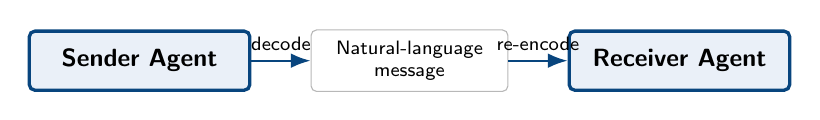
\begin{tikzpicture}[node distance=0.65cm]
\node[box, minimum width=2.8cm] (a) {Sender Agent};
\node[smallbox, right=0.75cm of a, minimum width=2.5cm] (text) {Natural-language\\message};
\node[box, right=0.75cm of text, minimum width=2.8cm] (b) {Receiver Agent};
\draw[arrow] (a) -- node[above, font=\scriptsize]{decode} (text);
\draw[arrow] (text) -- node[above, font=\scriptsize]{re-encode} (b);
\end{tikzpicture}
\end{center}

\vspace{0.45em}
\textbf{\textcolor{WarnRed}{Text-only communication의 세 가지 한계}}
\vspace{0.2em}
\begin{enumerate}
  \item \textbf{High inference cost}\\
  모든 메시지마다 sender는 token을 생성하고, receiver는 그 token을 다시 encoding해야 한다.

  \item \textbf{Information loss during discretization}\\
  고차원 hidden state가 vocabulary token 하나로 압축된다.
  논문은 token의 정보량을 대략 \(15\)--\(17\) bits로 보고, hidden state는 훨씬 큰 capacity를 가진다고 설명한다.

  \item \textbf{Redundancy and ambiguity of natural language}\\
  자연어는 사람이 읽기 좋지만 장황하고, hedge 표현이나 모호한 지시어 때문에 task-relevant density가 낮을 수 있다.
\end{enumerate}
\end{frame}

\begin{frame}[t]{Natural language vs. Latent communication: 언제 무엇을 쓰나?}
\footnotesize
\textbf{Latent communication이 natural language를 완전히 대체하는 것은 아니다.}
\vspace{1.25em}

\begin{columns}[T,onlytextwidth]
\begin{column}{0.49\textwidth}
\fcolorbox{DeepBlue}{SoftBlue}{\parbox{0.93\linewidth}{
\centering\textbf{Natural Language Communication}
\vspace{0.15em}
}}

\vspace{0.3em}
\textbf{자연어를 사용해야 하는 경우}
\begin{itemize}
  \item \textbf{사람의 해석이 필요할 때}
  \item 자연어 message는 사람이 즉시 읽을 수 있음
  \item debugging, alignment auditing, safety review에 유리
  \item human--AI interaction에서 그대로 설명하고 검토 가능
\end{itemize}

\textbf{사용할 때}
\begin{itemize}
  \item final answer를 제공할 때
  \item 사용자에게 justification을 보여줘야 할 때
  \item human oversight / cross-organization interoperability 필요
\end{itemize}

\end{column}

\begin{column}{0.49\textwidth}
\fcolorbox{GoodGreen}{SoftGreen}{\parbox{0.93\linewidth}{
\centering\textbf{Latent Communication}
\vspace{0.15em}
}}

\vspace{0.3em}
\textbf{Latent를 선호하는 경우}
\begin{itemize}
  \item \textbf{강하게 연결된 agents}\\
  planner \(\rightarrow\) executor처럼 바로 이어지는 agents
  \item \textbf{중간 communication}\\
  사용자가 message를 볼 필요가 없는 단계
  \item \textbf{공유되거나 정렬된 latent space}\\
  same backbone 또는 compatible architectures
  \item \textbf{latency가 핵심 제약인 경우}\\
  real-time pipeline, edge deployment, large agent counts
\end{itemize}

\end{column}
\end{columns}

\end{frame}

\begin{frame}[t]{무엇이 달라질 수 있나?}
\small
\textbf{핵심 아이디어:} agent가 자연어를 생성하지 않고 내부 연속 표현을 직접 전달한다.

\vspace{0.45em}
\begin{center}
\begin{tikzpicture}[node distance=0.75cm]
\node[box, minimum width=2.5cm] (sender) {보내는 agent};
\node[greenbox, right=0.8cm of sender, minimum width=3.0cm] (latent) {Embedding\\Hidden State\\KV-Cache};
\node[box, right=0.8cm of latent, minimum width=2.5cm] (receiver) {받는 agent};
\draw[arrow] (sender) -- (latent);
\draw[arrow] (latent) -- (receiver);
\node[redbox, below=0.7cm of latent, minimum width=5.6cm] (skip) {vocabulary bottleneck 우회};
\draw[redarrow] (skip) -- (latent);
\end{tikzpicture}
\end{center}

\vspace{0.4em}
\textbf{이 논문의 3-axis 분석 틀}
\vspace{0.2em}
\begin{columns}[T,onlytextwidth]
\begin{column}{0.32\textwidth}
\fcolorbox{DeepBlue}{SoftBlue}{\parbox{0.9\linewidth}{\centering
\textbf{WHAT}\\
무엇을 보낼까?\\
\scriptsize Embedding / Hidden State / KV-Cache
}}
\end{column}
\begin{column}{0.32\textwidth}
\fcolorbox{DeepBlue}{SoftBlue}{\parbox{0.9\linewidth}{\centering
\textbf{WHICH}\\
어디에 맞출까?\\
\scriptsize layer / latent alignment
}}
\end{column}
\begin{column}{0.32\textwidth}
\fcolorbox{DeepBlue}{SoftBlue}{\parbox{0.9\linewidth}{\centering
\textbf{HOW}\\
어떻게 합칠까?\\
\scriptsize concatenate / prepend / fuse
}}
\end{column}
\end{columns}

\vspace{0.45em}
\begin{center}
\fcolorbox{LineGray}{white}{\parbox{0.82\linewidth}{\centering
\[
\text{Method}
=(
\underbrace{\text{WHAT}}_{\text{type of information}},
\underbrace{\text{WHICH}}_{\text{alignment}},
\underbrace{\text{HOW}}_{\text{fusion}}
)
\]
}}
\end{center}
\end{frame}

\begin{frame}[plain]
\begin{tikzpicture}[remember picture,overlay]
  \node at (current page.center) {%
    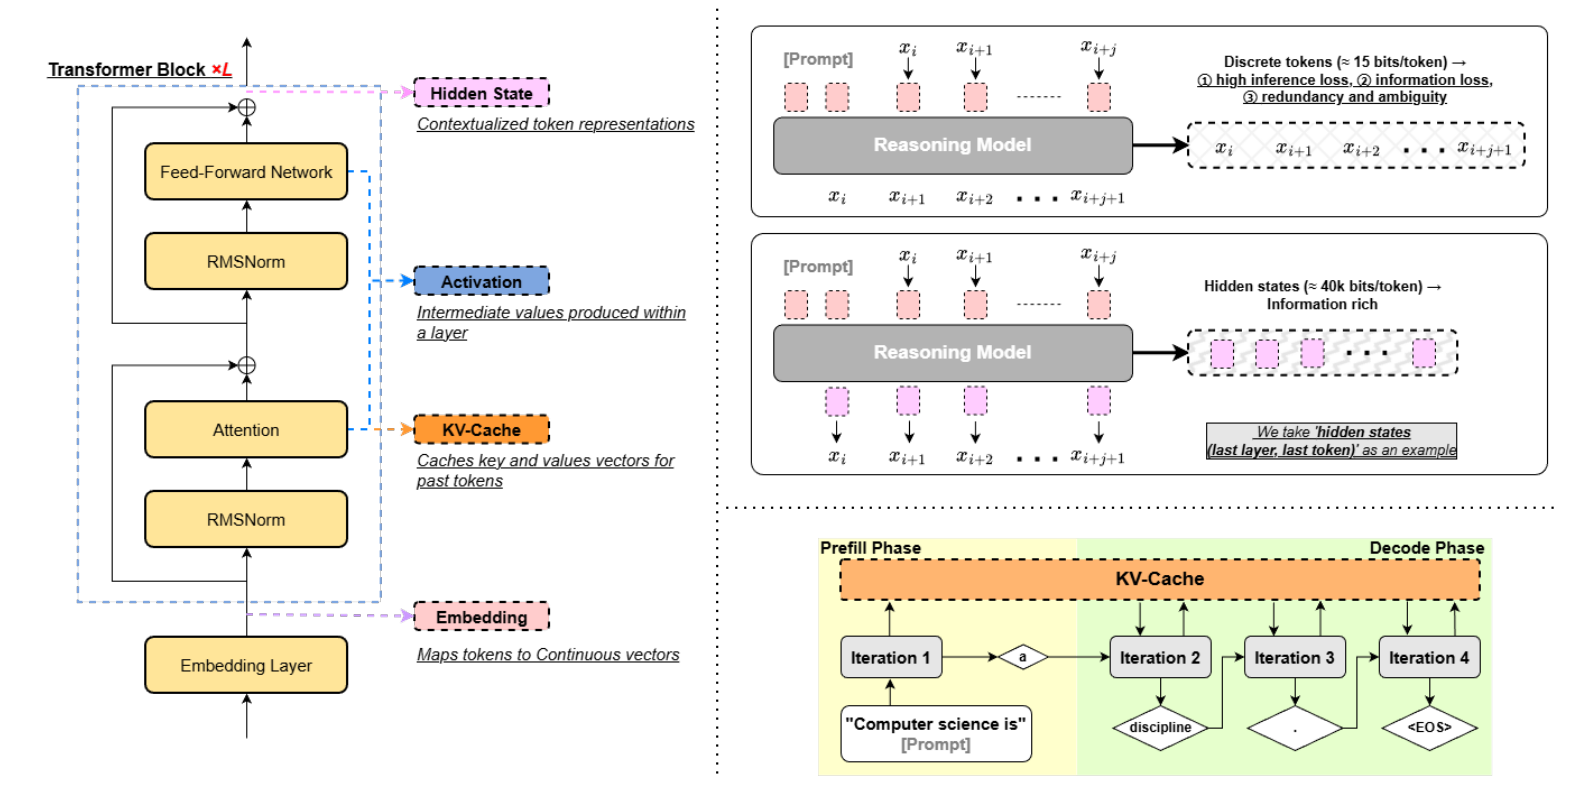
\includegraphics[width=0.99\paperwidth,height=0.96\paperheight,keepaspectratio]{figures/overview.png}%
  };
\end{tikzpicture}
\end{frame}

\begin{frame}[t]{WHAT: 어떤 정보를 전달할까?}
\small
\begin{columns}[T,onlytextwidth]
\begin{column}{0.48\textwidth}
\vspace{-0.4em}
\begin{center}
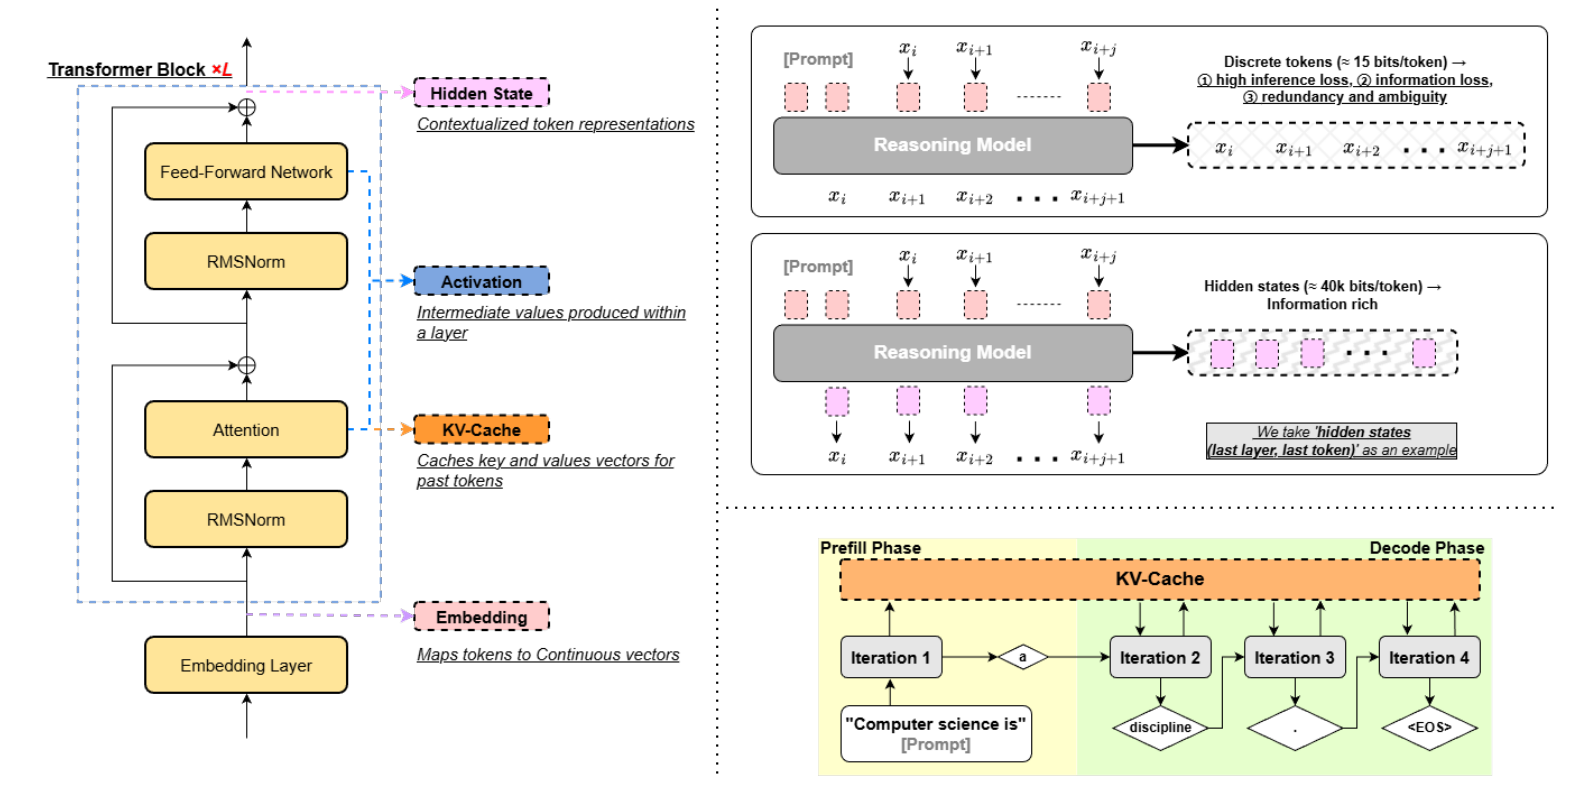
\includegraphics[
  width=\linewidth,
  height=0.74\textheight,
  keepaspectratio,
  trim=0 20 860 20,
  clip
]{figures/overview.png}
\end{center}
\end{column}

\begin{column}{0.49\textwidth}
\textbf{\textcolor{DeepBlue}{Embedding}}
\begin{itemize}
  \item 입력 token \(x_i\)를 dense vector로 바꾼 것
  \item 첫 Transformer block에 들어가는 가장 낮은 수준의 연속 표현
\end{itemize}
\[
e_i \in \mathbb{R}^d
\]

\vspace{0.25em}
\textbf{\textcolor{DeepBlue}{Hidden State}}
\begin{itemize}
  \item token \(i\)가 layer \(l\)의 Transformer block을 지난 출력
  \item attention과 문맥이 반영된 layer-wise semantic representation
\end{itemize}
\[
h_i^{(l)} \in \mathbb{R}^d
\]

\vspace{0.25em}
\textbf{\textcolor{DeepBlue}{KV-Cache}}
\begin{itemize}
  \item self-attention layer에서 token별 key/value를 저장한 것
  \item receiver가 sender context에 다시 attention할 수 있게 해주는 memory
\end{itemize}
\[
KV=\{(k_i^{(l)},v_i^{(l)})\}_{i=1,l=1}^{T,L}
\]
\end{column}
\end{columns}
\end{frame}

\begin{frame}[t]{WHICH: sender와 receiver를 어디서 맞출까?}
\small
\textbf{두 종류의 alignment가 있다.}

\vspace{0.35em}
\begin{columns}[T,onlytextwidth]
\begin{column}{0.48\textwidth}
\textbf{\textcolor{DeepBlue}{Latent information alignment}}
\begin{itemize}
  \item 같은 model이면 latent space가 거의 동일하다.
  \item 같은 backbone의 fine-tune이면 projection head를 쓸 수 있다.
  \item heterogeneous architecture이면 universal codec, interaction layer 등 learned alignment가 필요하다.
\end{itemize}
\end{column}
\begin{column}{0.48\textwidth}
\textbf{\textcolor{DeepBlue}{Layer alignment}}
\begin{itemize}
  \item \textbf{Last \(\rightarrow\) First}: sender last layer를 receiver first layer로.
  \item \textbf{All \(\rightarrow\) Corresponding}: sender layer \(l\)을 receiver layer \(l\)로.
  \item \textbf{Selected \(\rightarrow\) Selected}: 중요한 일부 layer만 선택.
\end{itemize}
\end{column}
\end{columns}

\vspace{0.45em}
\begin{center}
\fcolorbox{WarnRed}{SoftRed}{\parbox{0.86\linewidth}{\centering
같은 backbone에서는 training-free alignment가 가능하지만,
cross-architecture latent communication은 아직 어려운 open problem이다.
}}
\end{center}
\end{frame}

\begin{frame}[t]{HOW: receiver computation에 어떻게 합칠까?}
\scriptsize
\begin{adjustbox}{width=\linewidth}
\begin{tabular}{p{2.7cm}p{5.7cm}p{4.1cm}}
\toprule
HOW & Mechanism & Trade-off \\
\midrule
Concatenation &
sender latent를 receiver prompt embedding 또는 hidden state token axis에 붙인다. &
가장 단순하고 흔한 방식. hidden-state method에 잘 맞음. \\
\addlinespace
Prepending &
sender KV를 receiver KV-cache 앞에 붙인다. receiver가 sender context에 attention할 수 있다. &
KV-cache method의 자연스러운 fusion. long context에서 유리. \\
\addlinespace
Mathematical operation &
addition, subtraction, linear projection, gated combination 등으로 합친다. &
concat보다 expressive하지만 shape과 latent space compatibility가 필요. \\
\addlinespace
Cross-attention &
receiver가 sender latent set에 learned attention을 수행한다. &
가장 expressive하지만 training이 필요. MoT 계열. \\
\addlinespace
Cache restoration &
sender KV-cache를 receiver cache로 직접 복원/교체해 recomputation을 피한다. &
가장 효율적일 수 있지만 적용 범위가 제한적. \\
\bottomrule
\end{tabular}
\end{adjustbox}

\vspace{0.45em}
\begin{center}
\fcolorbox{DeepBlue}{SoftBlue}{\parbox{0.86\linewidth}{\centering
정리하면, latent communication 방법은
\textbf{무엇을 보내고(WHAT), 어디에 맞추고(WHICH), 어떻게 합치는지(HOW)}로 설명된다.
}}
\end{center}
\end{frame}

\begin{frame}[t]{Empirical insights: 무엇이 잘 먹히나?}
\vspace{2.4em}
\Large
\begin{center}
\begin{minipage}{0.86\linewidth}
\begin{enumerate}
  \item \textbf{\textcolor{DeepBlue}{Long context일수록 이득이 큼}}\\
  \normalsize receiver가 긴 prompt를 다시 encoding하지 않아도 되기 때문.

  \vspace{1.0em}
  \Large
  \item \textbf{\textcolor{DeepBlue}{Same-model agents가 지배적}}\\
  \normalsize 대부분 sender와 receiver가 같은 backbone을 공유한다고 가정.

  \vspace{1.0em}
  \Large
  \item \textbf{\textcolor{DeepBlue}{KV-cache가 emerging default}}\\
  \normalsize 18개 방법 중 9개가 KV-cache를 communicated quantity로 사용.
\end{enumerate}

\vspace{1.0em}
\large
\textbf{\textcolor{WarnRed}{핵심 trade-off}}:
정보량이 많을수록 latency는 줄기 쉽지만,
payload와 architecture dependence는 커진다.
\end{minipage}
\end{center}
\end{frame}

\end{document}
